%
% Annual Cognitive Science Conference
% Sample LaTeX Paper -- Proceedings Format
%

% Original : Ashwin Ram (ashwin@cc.gatech.edu)       04/01/1994
% Modified : Johanna Moore (jmoore@cs.pitt.edu)      03/17/1995
% Modified : David Noelle (noelle@ucsd.edu)          03/15/1996
% Modified : Pat Langley (langley@cs.stanford.edu)   01/26/1997
% Latex2e corrections by Ramin Charles Nakisa        01/28/1997
% Modified : Tina Eliassi-Rad (eliassi@cs.wisc.edu)  01/31/1998
% Modified : Trisha Yannuzzi (trisha@ircs.upenn.edu) 12/28/1999 (in process)
% Modified : Mary Ellen Foster (M.E.Foster@ed.ac.uk) 12/11/2000
% Modified : Ken Forbus                              01/23/2004
% Modified : Eli M. Silk (esilk@pitt.edu)            05/24/2005
% Modified : Niels Taatgen (taatgen@cmu.edu)         10/24/2006
% Modified : David Noelle (dnoelle@ucmerced.edu)     11/19/2014

%% Change "letterpaper" in the following line to "a4paper" if you must.

%%% MAX = 6 Pages (including references)

\documentclass[10pt,letterpaper]{article}

\usepackage{cogsci}
\usepackage{pslatex}
\usepackage{graphicx}
\usepackage{apacite}
\usepackage{color}


\title{Word Identification Under Multimodal Uncertainty}

\author{{\large \bf Abdellah Fourtassi} \\ afourtas@stanford.edu \\
  Department of Psychology\\ Stanford University\\
  \And {\large \bf Michael C. Frank}\\ mcfrank@stanford.edu \\
  Department of Psychology\\ Stanford University}


\begin{document}

\maketitle


\begin{abstract}

Identifying the visual referent of a spoken word -- that a particular insect is referred to by the word ``bee'' -- requires both the ability to process and integrate multi-modal input and the ability to identify categories under uncertainty. How do these tasks interact with one another? We introduce a task that allows us to examine how adults identify word categories under joint uncertainty in the auditory and visual modalities. We propose a Bayesian model of the task which provides an optimal baseline. Model predictions are tested in two experiments where category recognition is made under two kinds of uncertainty: ambiguity and noise. In both cases, the optimal baseline model explains much of the variance in human judgments. But when one modality had noise added to it, human perceivers systematically preferred the unperturbed modality to a greater extent than the optimal baseline model did.

\textbf{Keywords:}
Language; audio-visual processing; word learning; speech perception; computational modeling.
\end{abstract}

 % (e.g., the visual modality in the case of concrete objects)
Language uses symbols expressed in one modality (e.g., the auditory modality, in the case of speech) to communicate about the world, which we perceive through many different sensory modalities. Consider hearing someone yell ``bee!" at a picnic, as a honeybee buzzes around the food. Determining reference involves processing the auditory information and linking it with other perceptual signals (e.g., the visual image of the bee, the sound of its wings, the sensation of the bee flying by your arm). But processing this linguistic input also requires categorization. On the linguistic side,  individual sounds must be identified as members of phonetic categories for the word to be understood. On the referential side, individual sensory impressions must be categorized as coming from a bee. Once these two sets of category-identification tasks have been completed, then a listener can make the referential link between word and world.

This comprehension task takes place in a noisy world. On the auditory side, individual acoustic word tokens are almost always ambiguous with respect to the particular sequence of phonemes they represent \cite<e.g.,>{hillenbrand1995}. And some tokens may be distorted additionally by mispronunciation or ambient noise. Perhaps the speaker was yelling ``pea" and not ``bee.'' Similarly, a sensory impression may not be enough to make a definitive identification of a visual category.\footnote{In the general case, language can of course be visual as well as auditory, and object identification can be done through many modalities. For simplicity, we focus on audio-visual matching here.} Perhaps the quickly flying insect was a beetle or a fly instead.

Thus, establishing reference requires reasoning under a great deal of uncertainty. Work on phoneme categorization has suggested that perceivers encode tokens probabilistically: they base their decisions on these probabilities and adjust their behavior when these probabilities change \cite<e.g.,>{clayard08}. However, previous work in this line of research has largely focused on the unimodal case, that is, when category uncertainty is only in one modality \cite<e.g.,>{feldman2009}. A few studies have explored some aspects of cross-modal processing  \cite<e.g.,>{bejjanki2011, kleinschmidt2015}. This work has focused on the specific case of phoneme recognition from speech and lip movement, however, where information from both modalities is tightly correlated.

In the present work, we study the case of word recognition, where a word is an \textit{arbitrary} mapping between a sound category and a visual category. We test participants on their ability to process audio-visual stimuli and use them to recognize the underlying word category. Crucially, this recognition is made under uncertainty about both the auditory category (a single phoneme, in our case) and the visual category (the concept being referred to). Our goal is to explore how adults deal with such multimodal ambiguity in a categorization task. To this end, we propose a model that combines uncertainty in an optimal way, and we use it as a baseline for interpreting human data. More precisely, we examine the extent to which human data conform to, or deviate from the baseline, and whether the deviation involves a systematic preference for a particular modality.

The paper is organized as follows. First, we introduce our audio-visual word recognition task. We next present the model and explain how it provides an optimal baseline. Then we present two behavioral experiments where we test category recognition under audio-visual uncertainty. In Experiment 1, audio-visual tokens are clear but their category membership is ambiguous. In Experiment 2, we intervene by adding additional perceptual noise to one modality. While participants show no modality preference in Experiment 1, in Experiment 2 they over-rely on visual input when the auditory modality is noisy.

\section{The Audio-Visual Word Recognition Task}

We introduce a new task that tests audio-visual category recognition. We use two visual categories (cat and dog) and two auditory categories (/b/ and /d/ embedded in the minimal pair /aba/-/ada/). For each participant, an arbitrary pairing is set between the auditory and the visual categories, leading to two audio-visual word categories (e.g., dog-/aba/, cat-/ada/).

In each trial, participants are presented with an audio-visual target (the prototype of the target category), immediately followed by an audio-visual test stimulus (Figure \ref{fig:task}). The test stimulus may differ from the target in both the auditory and the visual components. The auditory component is sampled from a continuum along the second formant (F2) linking the words /aba/ and /ada/. The visual component is sampled from a morph that links the prototypical pictures of the dog and the cat.  After these two presentations, participants are instructed to press ``same'' or ``different.''

This task is similar to the task introduced by \citeA{sloutsky2003} and used in subsequent research to probe audio-visual encoding. However, unlike this previous line of research, here participants are not asked whether the two audio-visual presentations are identical. Instead, the task is category-based: They are asked to press `same' if they think the second item (the test) belonged to the same category as the first (e.g.,  dog-/aba/), even if there is a slight difference in the word, in the object, or in both. They are instructed to press `different' only if they think that the second stimulus was an instance of the other word category (cat-/ada/).

The task also included trials where pictures were hidden (audio-only) or where sounds were muted (visual-only). These unimodal trials provide us with participants' categorization functions for the auditory and visual categories and are used as inputs to the optimal model, described below.

\begin{figure}[tp]
\centering
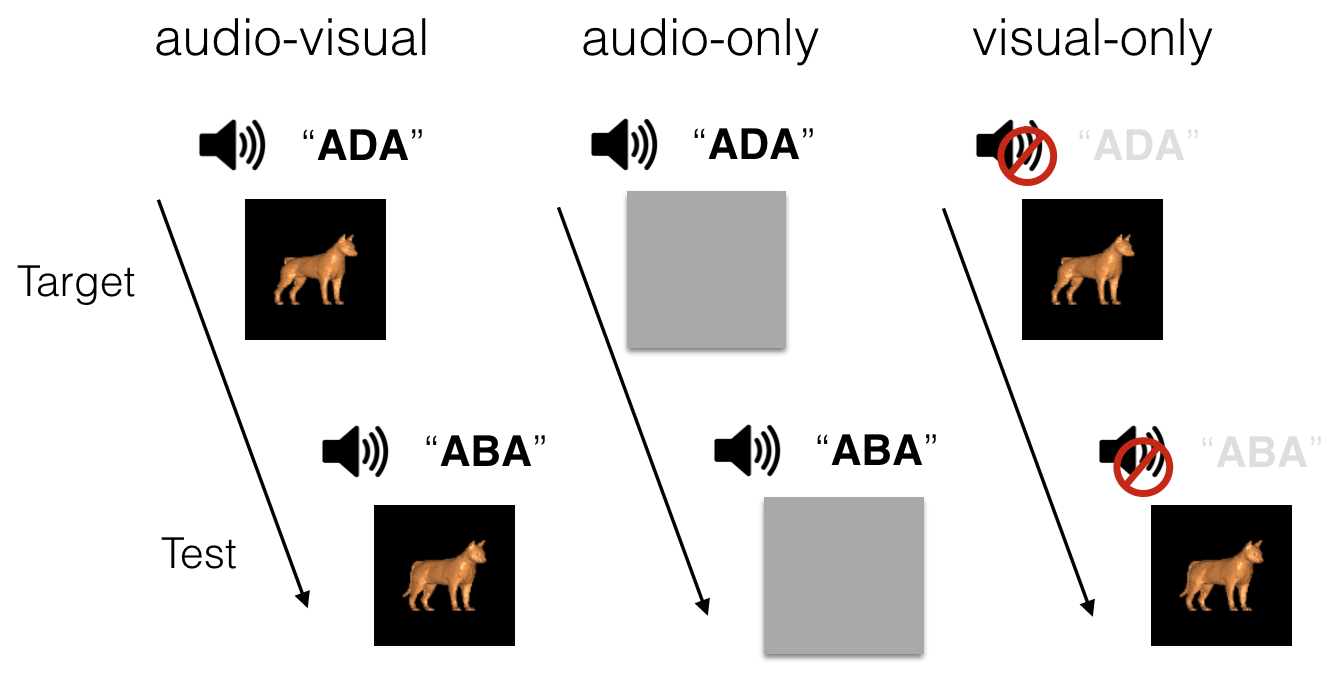
\includegraphics[width=0.4\textwidth]{task1.png}
\caption{Overview of the task}
\label{fig:task}
\end{figure}

\section{Ideal Observer Model}

The basis of our ideal observer model is that individual categorization functions from each modality should be combined optimally.
In each modality, we have two categories: /ada/ ($A=1$) and /aba/ ($A=2$) in the auditory dimension, and \textit{cat} ($V=1$) and \textit{dog} ($V=2$) in the visual dimension.
% \footnote{The identity of the categories was randomized in the experimental setup.}
We assume, for the sake of simplicity, that the probability of membership in each category is normally distributed:

$$ p(a | A) \sim  N(\mu_A, \sigma^2_A) $$
$$ p(v | V) \sim  N(\mu_V, \sigma^2_V) $$

In the bimodal condition, participants see word tokens with audio-visual input, and have to make a categorization decision. We represent word tokens as vectors in the audio-visual space, $\mathbf{w}=(a,v)$.
A word category $W$ is defined as the joint distribution of auditory and visual categories. It can be characterized with a bivariate normal distribution in the audio-visual space:
$$ p(\mathbf{w} | W) \sim  N(M_W, \Sigma_W) $$

\begin{figure}[tp]
  \centering
  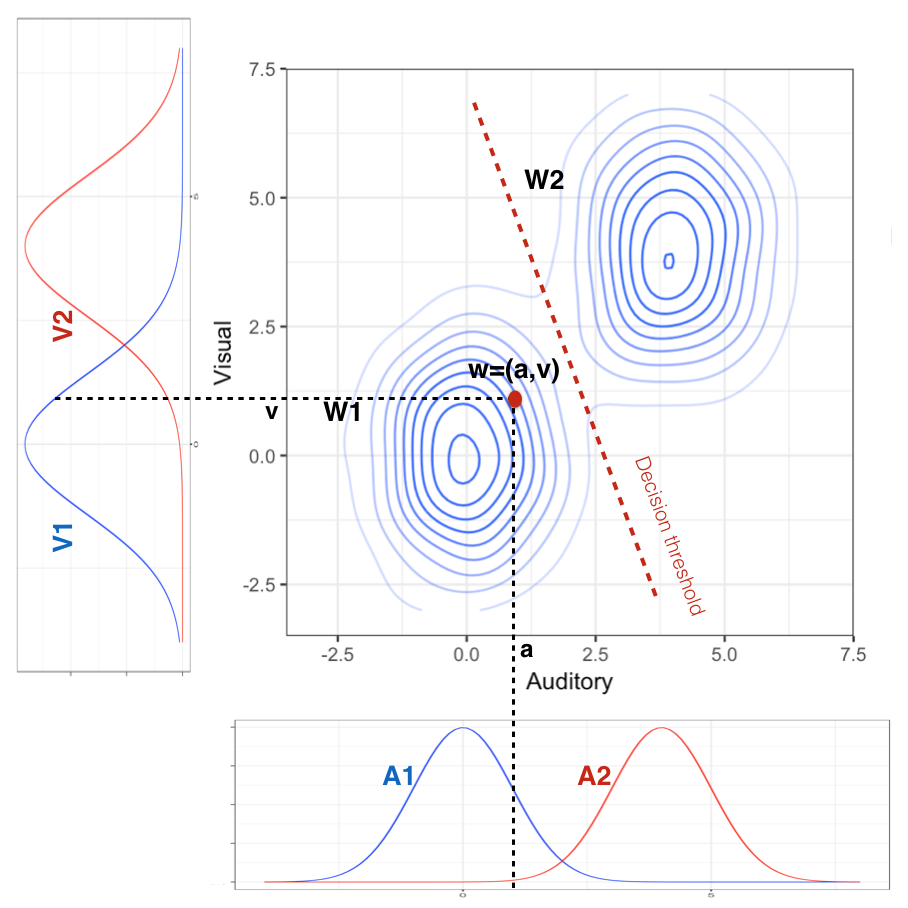
\includegraphics[width=3.25in]{MyTask.png}
  \caption{Illustration of our model using simulated data. A word category is defined as the joint bivariate distribution of an auditory category (horizontal, bottom panel) and a visual semantic category (vertical, left panel). Upon the presentation of a word token $w$, participants guess whether it is sampled from the word category $W_1$ or from $W_2$. Decision threshold is where the guessing probability is 0.5.}
  \label{fig:space}
\end{figure}

We have two word categories: dog-/aba/ ($W_1$) and cat-/ada/ ($W_2$). Participants can be understood as choosing one of these two word categories (figure \ref{fig:space}). For an ideal ``recognizer'', the probability of choosing category 2 when presented with an audio-visual instance $\mathbf{w}=(a,v)$ is the posterior probability of this category:

\begin{equation}
% \small
p(W_2 | \mathbf{w})=\frac{p(\mathbf{w}|W_2)p(W_2)}{p(\mathbf{w}|W_2)p(W_2)+p(\mathbf{w}|W_1)p(W_1)}
\end{equation}

We make the assumption that, given a particular word category, the auditory and visual tokens are independently generated:

\begin{equation}
p(\mathbf{w} | W) = p(a,v| W) = p(a| W)p(v| W)
\end{equation}

Under this assumption, the posterior probability reduces to:
\begin{equation}
p(W_2 | \mathbf{w})=\frac{1}{1+(1+\epsilon)\exp(\beta_0+\beta_aa+\beta_vv)}
\label{eq:pred}
\end{equation}

with $\beta_a=\frac{\mu_{A1}-\mu_{A2}}{\sigma^2_{A}}$,
$\beta_v=\frac{\mu_{V1}-\mu_{V2}}{\sigma^2_{V}}$,
$\beta_0=\frac{\mu^2_{A2}-\mu^2_{A1}}{2\sigma^2_{A}}+\frac{\mu^2_{V2}-\mu^2_{V1}}{2\sigma^2_{V}}$

and $1+\epsilon=\frac{p(W_1)}{p(W_2)}$ is the proportion of the prior probabilities. If the identity of word categories is randomized, and if $W_1$ is the target, then $\epsilon$ measures a response bias to ``same'' if $\epsilon > 0 $, and a response bias to ``different'' if $\epsilon < 0 $.

In sum, the posterior \ref{eq:pred} provides a baseline for how probabilities that characterize uncertainty in each modality can be combined to make categorical decision about bimodal input.


\section{Experiment 1}

In experiment 1, we test the predictions of the model in the case where uncertainty is due to perceptual ambiguity in terms of category membership. This experiment had two goals. First, we wanted to examine the extent to which human responses corresponded to the predictions of the ideal observer model. Second, if there was a deviation from the baseline, we wanted to be able to measure whether this deviation involved a systematic preference for a particular modality.

\subsection{Methods}

\subsubsection{Participants}

We recruited a planned sample of 100 participants, recruited from Amazon Mechanical Turk. Only participants with US IP addresses and a task approval rate above 85\% were allowed to participate. They were paid at an hourly rate of \$6/hour. Data were excluded if participants completed the task more than
once (2 participants). Moreover, as specified in the preregistration (\url{https://osf.io/h7mzp/}), participants were excluded if they had less than 50\% accurate responses on the unambiguous training trials (6), and if they reported having experienced a technical problem of any sort during the online experiment (14). The final sample consisted of 76 participants.

\subsubsection{Stimuli}

For  auditory stimuli, we used the continuum introduced in \citeA{vroomen2004}, a 9-point /aba/--/ada/ speech continuum created by varying the frequency of the second (F2) formant in equal steps. We selected 5 equally spaced points from the original continuum by keeping the end-points (prototypes) 1 and 9, as well as points 3, 5, and 7 along the continuum. For visual stimuli, we used a morph continuum introduced in \citeA{freedman2001}: a continuous set of images was generated from three cat prototypes and three dog prototypes. From the original 14 points, we selected 5 points as follows: we kept the item that seemed most ambiguous (point 8), the 2 preceding points (i.e., 7 and 6) and the 2 following points (i.e., 8 and 9). The 6 and 9 points along the morph were quite distinguishable, and we took them to be our prototypes.

 % (Figure \ref{fig:morph})
%
% \begin{figure}[tp]
% \centering
% 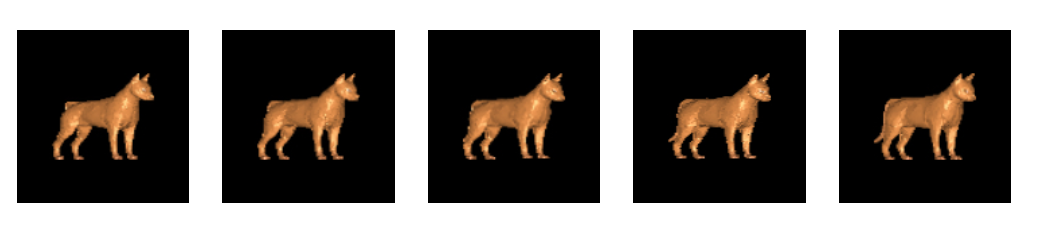
\includegraphics[width=0.4\textwidth]{morph.png}
% \caption{Visual stimuli for our experiments.}
% \label{fig:morph}
% \end{figure}

\subsubsection{Design and Procedure}

We told participants that an alien was naming two objects: a dog, called /aba/ in the alien language, and a cat, called /ada/. In each trial, we presented the first object (the target) on the left side of the screen simultaneously with the corresponding sound. The target was always the same (e.g., dog-/aba/). The second sound-object pair (the test) followed on the other side of the screen after 500ms and varied in its category membership. For both the target and the test, visual stimuli were present for the duration of hte sound clip ($\sim$800ms). We instructed participants to press ``S'' for same if they thought the alien was naming another dog-/aba/, and ``D'' for different if they thought the alien was naming a cat-/ada/. For each participant, we randomized the sound-object mapping as well as the identity of the target.

The first part of the experiment trained participants using only the prototype pictures and the prototype sounds (12 trials, 4 each from the bimodal, audio-only, and visual-only conditions). After completing training, we instructed participants on the structure of the task and encouraged them to base their answers on both the sounds and the pictures (in the bimodal condition). There were a total of 25 possible combinations in the bimodal condition, and 5 in each of the unimodal conditions. Each participant saw each possible trial in each condition twice, for a total of 70 trials/participants. Trials were blocked by condition and blocks were presented in random order.
% We designed the experiment to take between 10 to 15 minutes to complete.

\begin{figure}
\centering
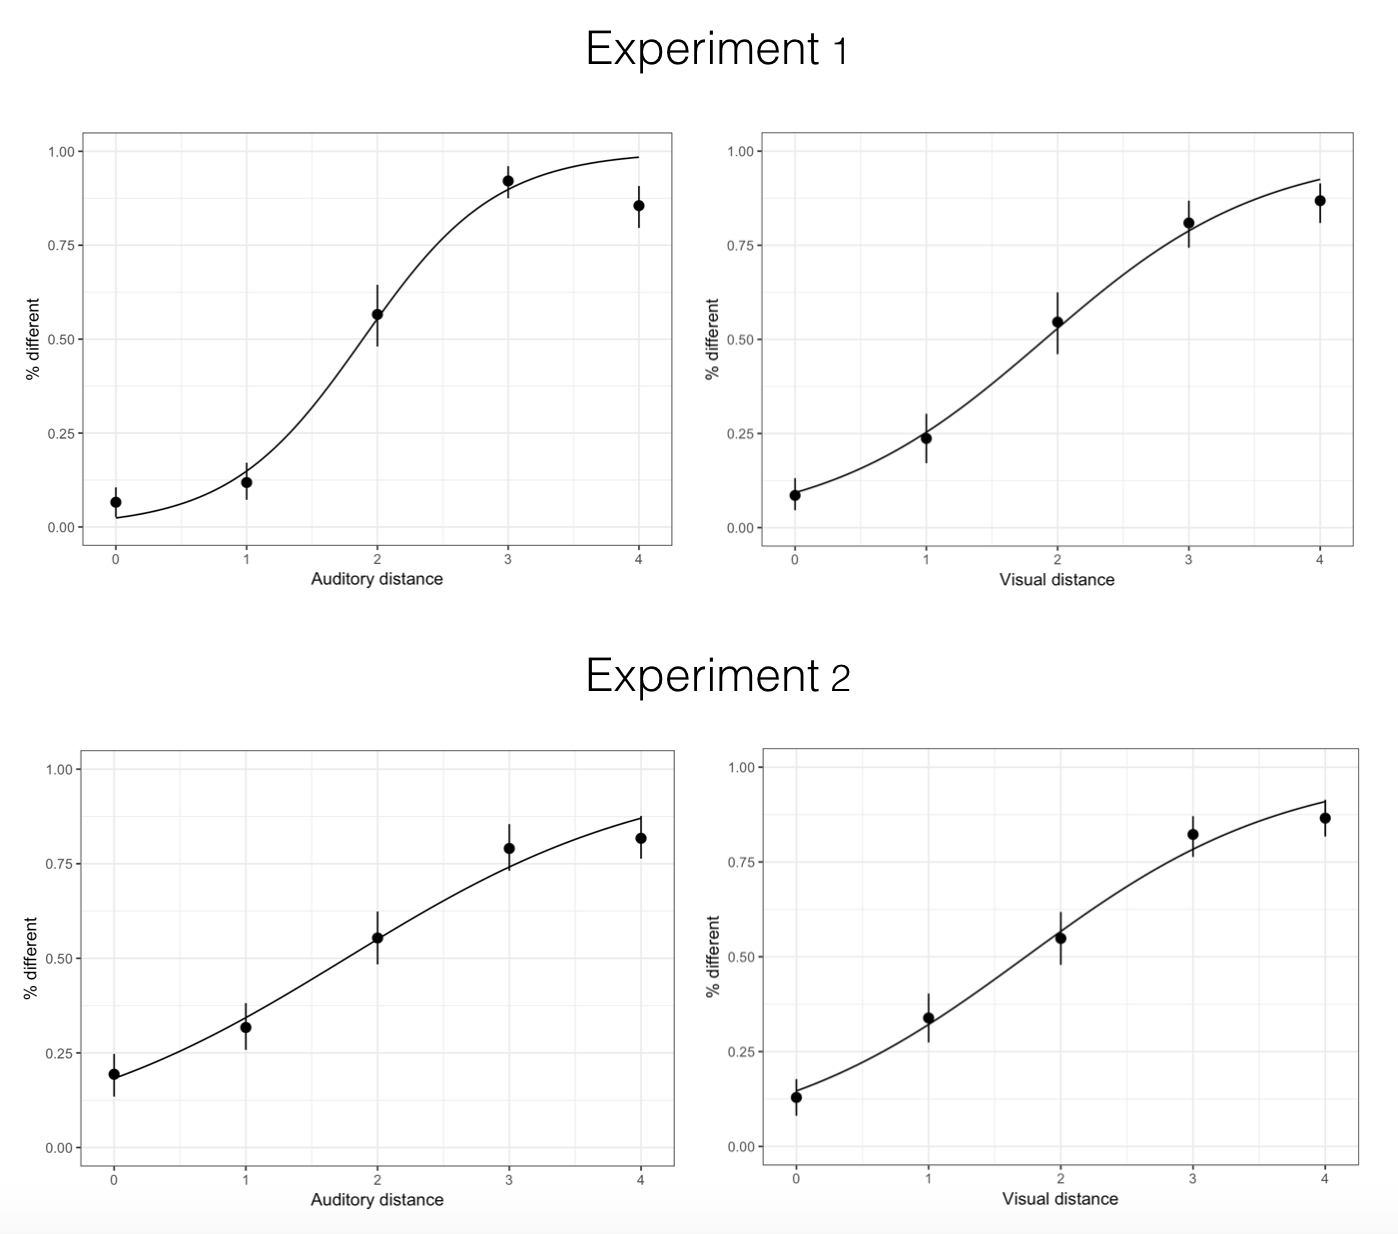
\includegraphics[width=3.25in\textwidth]{unimodal.png}
\caption{Average human responses in the auditory-only condition (left), and visual-only condition (right). Error bars are 95\% confidence intervals. Solid lines represent unimodal logistic fits.}
\label{fig:unimodal}
\end{figure}


\subsection{Results}
%
% \begin{figure}[h]
% \centering
% 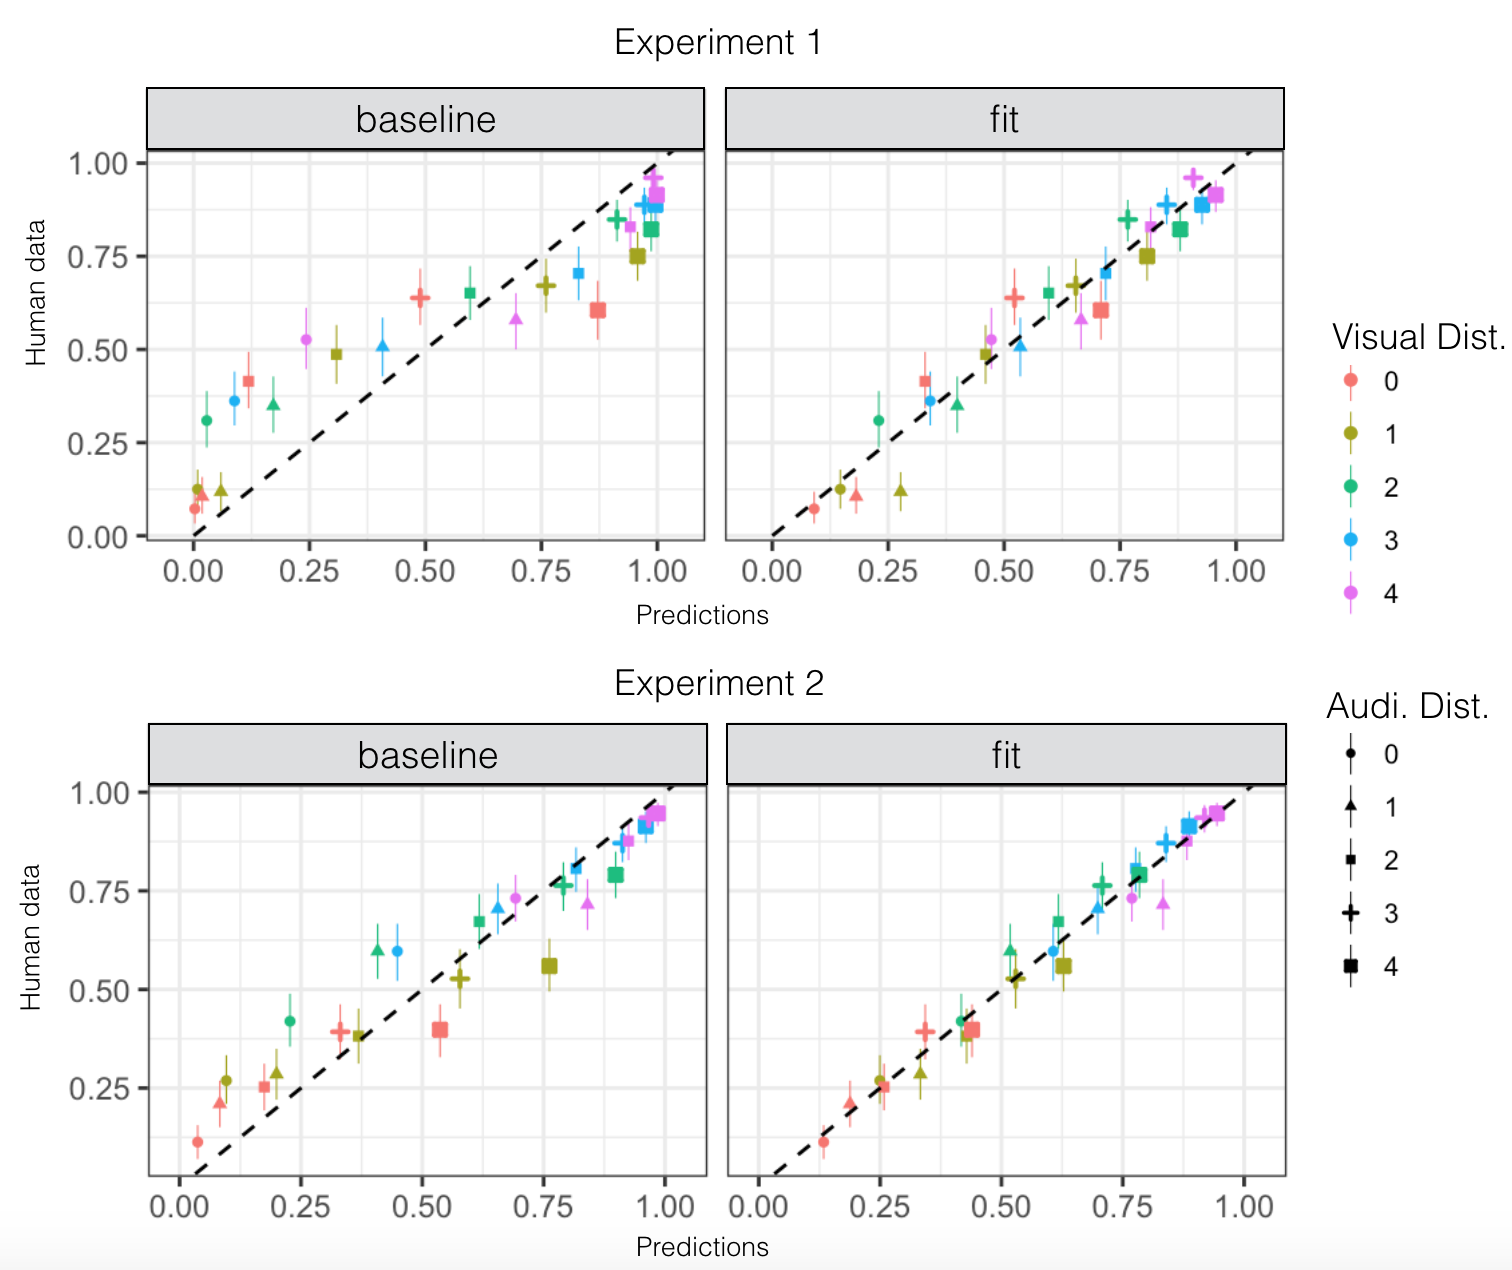
\includegraphics[width=3.25in\textwidth]{correlation.png}
% \caption{Human responses vs. the baseline predictions. Error bars are 95\% confidence intervals. In experiment 1, the baseline and the fit explained 89\%, and 94\% of total variance, respectively. In experiment 2, the baseline and the fit explained 91\%, and 97\% of total variance, respectively}
% \label{fig:corr}
% \end{figure}

\begin{figure*}[t]
\centering
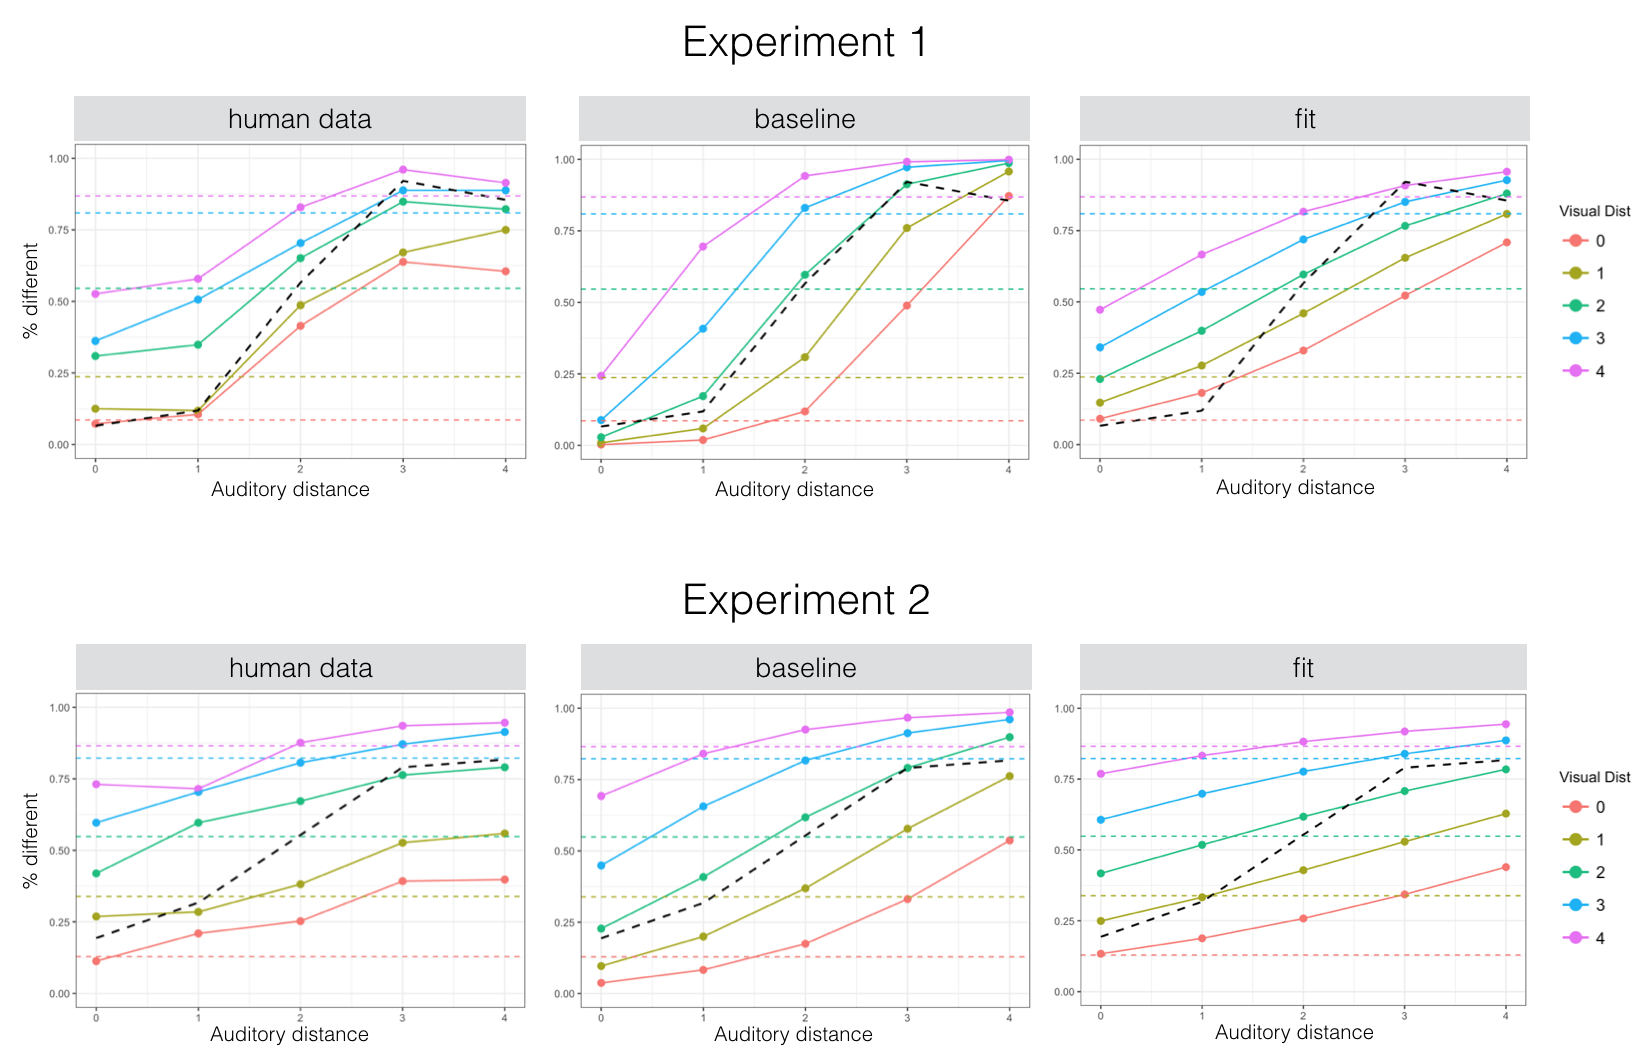
\includegraphics[width=.83\textwidth]{Exp.png}
\caption{Proportion of ``different'' judgments as a function of auditory distance. Solid lines represent average human responses (left), predictions of the baseline (middle), and the bimodal fit (left). Dashed lines represent average human responses in the unimodal conditions. Colors represent values in the visual continuum.}
\label{fig:Exp}
% \vspace{10ex}
\end{figure*}

% Let's take the auditory-only case as an example,
\subsubsection{Unimodal conditions}

Average categorization judgments and fits are shown in Figure \ref{fig:unimodal}. Auditory judgements were somewhat sharper and more pronounced than visual judgments. For an ideal recognizer, the probability of choosing category 2 (that is, to answer ``different'') when presented with e.g., an audio instance $a$, is the posterior probability of this category $p(A_2|a)$. If we assume that both categories have equal variances, the posterior probability reduces to:

\begin{equation}
p(A_2 | a)=\frac{1}{1+(1+\epsilon_A)\exp(\beta_{a0}+\beta_aa)}
\end{equation}

with $\beta_a=\frac{\mu_{A_1}-\mu_{A_2}}{\sigma^2_{A}}$ and  $\beta_{a0}=\frac{\mu^2_{A_2}-\mu^2_{A_1}}{2\sigma^2_{A}}$. $\epsilon_A$ is the response bias in the auditory-only trials.

For this model (as well all other models), we fixed the values of the means to be the end-points of the corresponding continuum: $\mu_{A1}=0$ and $\mu_{A2}=4$ (and similarly $\mu_{V1}=0$, and $\mu_{V2}=4$). To determine the values of the bias and the variance, we fit a model for each modality, collapsed across participants. For the auditory modality, we got $\epsilon_A=-0.20$ and $\sigma^2_A=2.04$. For the visual modality, we got $\epsilon_V=-0.11$ and $\sigma^2_V=3.34$.
% In figure \ref{fig:unimodal} (top) we plotted responses in the unimodal conditions as well as the unimodal fits.

\subsubsection{Bimodal condition}

We fit a model to human responses in the bimodal condition, collapsed across participants, finding $\epsilon=-0.32$, $\sigma^2_{Ab}=5.00$ and $\sigma^2_{Vb}=7.27$.

\subsubsection{Baseline model}

We derived the predictions of the baseline model by using the values of the variances derived from the unimodal conditions, and the response bias derived from the bimodal condition, and by substituting these values into the expression of the posterior in Eq.~\ref{eq:pred}. Figure \ref{fig:Exp} shows participants' responses in the bimodal condition (left), as well as the prediction of the baseline (middle), and the bimodal fit models (right).
% Correlation of human data and the bimodal baseline/fitted model are shown in Figure \ref{fig:corr} (top).

\subsubsection{Response bias}

We found negative values for in all response bias terms, which suggests a general bias toward answering ``different.''  This bias is probably due to the categorical nature of the task: when two items are ambiguous but perceptually different, this could cause a slight preference for ``different'' over ``same.''

\subsubsection{Modality preferences}

We next analyzed whether there was a preference for one or the other modality when making decisions in the bimodal condition, beyond that explained by the variance in categories implied by the unimodal responses. This preference would manifest as a deviation from the decision threshold predicted by the baseline model. The decision threshold is defined as the set of values in the audio-visual space along which the posterior (Eq.~\ref{eq:pred}) is equal to 0.5. The decision threshold takes the following form:
% As illustrated in \ref{fig:space}, above this line participants are more likely to choose one word category, and below this line, they are more likely to choose the other word category.

\begin{equation}
v=-\frac{\sigma^2_V}{\sigma^2_A}a+v_0
\label{eq:threshold}
\end{equation}

If the slope derived from the fit is bigger than the slope of the baseline, this finding would suggest a general preference for the auditory modality (similarly, a smaller slope would suggest a preference for the visual modality). The limit cases are when there is exclusive reliance on the auditory cue (a vertical line), and where there is exclusive reliance on the visual (a horizontal line). Figure \ref{fig:pref} (top left) shows the decision threshold in the audio-visual space with a constant intercept; the fit to human data  (solid black line) was very close to the baseline threshold (red line). Non-parametric resampling sampling of the data showed no evidence of a deviation from the baseline (\ref{fig:pref}, bottom left).

\subsection{Discussion}

% Compare human responses (figure \ref{fig:Exp}, top left) to the baseline (figure \ref{fig:Exp}, top middle).
Qualitatively, participants' judgments were similar to the predictions of the optimal baseline model (when fit to the unimodal data). Consider the contrast between the auditory-only case (dashed black line in Figure \ref{fig:Exp}, top left) and the bimodal case (solid colored lines).  Higher certainty in the visual modality generally influenced responses, with greater visual distance leading to more ``different'' ratings and less visual distance leading to more ``same'' ratings. Indeed, we found that the baseline model explained almost 90\% of the variance in judgments ($r^2=0.89$). In addition, as described above, we did not see any evidence for a modality preference.

But although we see a qualitative resemblance data and baseline model, there were quantitative differences. Model predictions were more influenced by the visual modality at the auditory midpoint (the point of highest uncertainty) than human judgements, and were more compressed at the endpoints (the points of lowest uncertainty). Formally speaking, this trend translated into an increase in the value of the variance associated with each modality (e.g., compare the variance values in the baseline model to the values derived from the bimodal fit).  Since the variance characterizes the reliability of a given cue, it seems as if bimodal presentation caused reliance on both modalities to decrease. This effect could possibly be attributed to the arbitrary nature of the form-meaning mapping. In fact, previous studies suggest that while redundant multi-modal information improves performance (e.g., determining the frequency of a bouncing ball from visual and auditory cues), arbitrary mappings generally tends to hinder performance \citeA<for review, see>{robinson2010}.


\section{Experiment 2}

In Experiment 1, we tested the ability of people to recognize a word category under ambiguous tokens. In particular, the tokens were clear but their category membership was uncertain. In real life situations, however, even the identity of the token can be uncertain due to various distorting factors. In order to account for this kind of uncertainty in the auditory modality, we can imagine \cite<following>{feldman2009}, that the speaker generates a target production $t$ from an auditory category
$t | A \sim N(\mu_{A}, \sigma^2_{A})$. The listener, in a noisy condition, does not hear exactly this produced target, but the target perturbed by normally distributed noise: $a | t \sim N(t, \sigma^2_{N})$. When we integrate over $t$, we get:

\begin{equation}
a | A \sim N(\mu_{A}, \sigma^2_{A}+\sigma^2_{N})
\end{equation}

In Experiment 2, we explored the effect of noise on performance in our task. We tested a case where one modality was ambiguous and noisy (auditory), and where the other modality was ambiguous but not noisy (visual). We were interested to know if participants would treat this new source of uncertainty as predicted by the optimal baseline, and whether noise in one modality would lead to some systematic preference for the non-noisy modality.

\subsection{Methods}

\subsubsection{Participants}

A planned sample of 100 participants was recruited online through Amazon Mechanical Turk. We used the same exclusion criteria as in the previous experiment; the final sample consisted of 93 participants.

\subsubsection{Stimuli and Procedure}

We used the same visual stimuli as in Experiment 1. We also used the same auditory stimuli , but we convolved each item with Brown noise of amplitude 1 using the audio editor Audacity (2.1.2). The procedure was exactly the same as in the previous experiment, except that target stimuli were presented with the new noisy auditory stimuli.

\subsection{Results}

\subsubsection{Unimodal conditions}

We fit a model for each modality, collapsed across participants. For the auditory modality, our parameter estimates were $\epsilon_A=-0.18$ and $\sigma^2_A+\sigma^2_N=4.70$. For the visual modality, we found $\epsilon_V=-0.24$ and $\sigma^2_V=3.93$.  Figure \ref{fig:unimodal} (bottom) shows responses in the unimodal conditions as well as the unimodal fits. In contrast to Experiment 1, auditory responses were flatter (showing more uncertainty).

\subsubsection{Bimodal condition}

We fit a model to human responses in the bimodal condition, collapsed across participants. We estimated $\epsilon=-0.38$, $\sigma^2_{Vb}=5.21$, and  $\sigma^2_{Ab}+\sigma^2_{Nb}=9.84$.

\subsubsection{Baseline model}

We generated the predictions of the baseline model by using the values of the variances derived from the unimodal conditions, and the response bias derived from the bimodal condition, and by plugging these values into Eq.~\ref{eq:pred}.
Results are shown in Figure \ref{fig:Exp} (bottom).
 % Correlation of human data to the bimodal baseline and the fit are shown in figure \ref{fig:corr} (bottom).

\subsubsection{Discussion}

\begin{figure}[h]
\centering
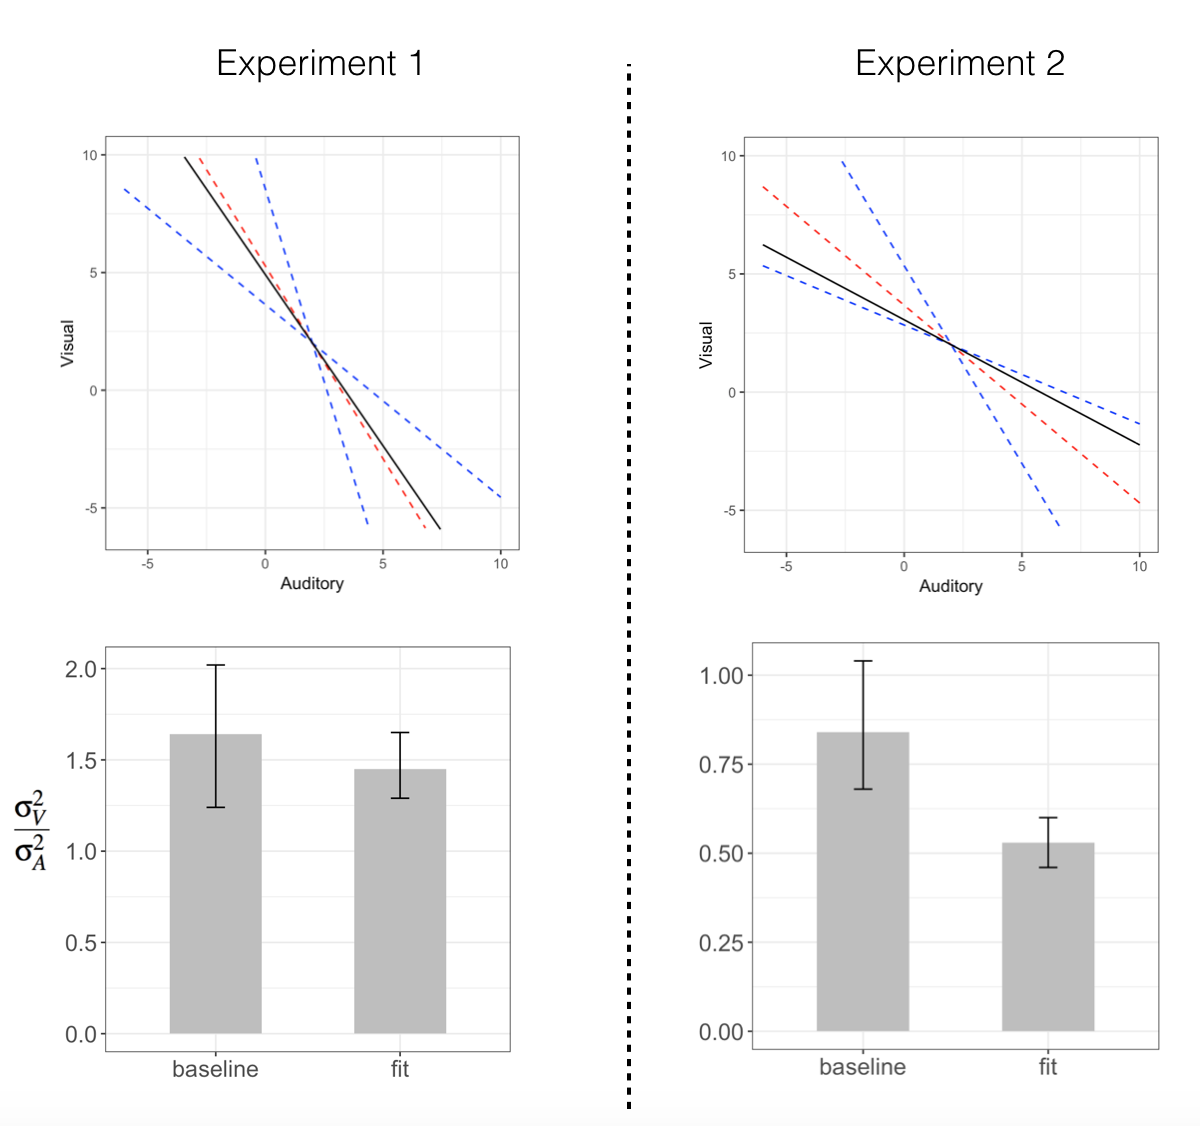
\includegraphics[width=0.4\textwidth]{preference.png}
\caption{Top: decision thresholds in the audio-visual space. Red dotted line is the prediction of the baseline. Blue dotted lines are cases where modality preference is twice as strong as the baseline. Solid line is the threshold derived from human data. Bottom: comparison of the threshold slope between the baseline and the fit to human data. Error bars are 95\% confidence intervals computed through non-parametric bootstrap sampling (10.000 samples)}
\label{fig:pref}
\end{figure}

We found, similar to experiment 1, that participants generally showed qualitative patterns similar to the baseline model ($r^2 = .91$). But we also found a similar discrepancy at the quantitative level: There was a decrease in the reliability of both modalities, as could be inferred from the increase in the variance associated with the auditory modality and the visual modality in the bimodal fit. An interesting difference with Experiment 1, however, was that participants' decision threshold suggested a preference for the visual modality (the non-noisy modality). Indeed non-parametric bootstrap sampling over the data showed there to be a significant decrease in the value of the slope.

\section{Conclusion}

In this work, we tested word category recognition under audio-visual uncertainty. We modeled uncertainty as a probability distribution over tokens from auditory and visual continua. Our baseline model instantiated an ideal observer, optimally combining participant data from unimodal decisions. The model's predictions were examined in two experiments where we tested two kinds of uncertainty: in experiment 1, audio-visual tokens were clear but their category membership was ambiguous. In experiment 2, input to one modality was ambiguous, and input to the other was ambiguous as well as noisy. In both experiments, the ideal observer model explained the majority of variance in participant judgments. In both experiments, however, we found that bimodal presentation caused the reliability of both modalities to decrease relative to the ideal observer.

We explored whether part of the unexplained variance could involve to a systematic preference for a given modality. Our analysis showed no evidence of such modality preference in experiment 1. However, we found a preference for the non-noisy modality in experiment 2.

This paper addressed the problem of recognizing words whose underlying phonemic and semantic categories were supposed to be familiar. An intriguing challenge is to understand how these underlying categories are acquired in the first place. Previous developmental work addressed cases when one modality was supposed to provide a stable and certain cue to the other modality \cite<e.g.,>{waxman1995, yeung09}. The present paper invites investigations on category acquisition in the more general case where there is uncertainty in both modalities.






\bibliographystyle{apacite}

\setlength{\bibleftmargin}{.125in}
\setlength{\bibindent}{-\bibleftmargin}

\bibliography{CogSci_Template}


\end{document}
